% Instructions: after you type, run "latex example" (twice to get cross references to show
% correctly). Figures can be included as shown below. If figure is not available, latex
% will complain, press enter repeatedly until it goes through, or put a figure, or else
% comment out the lines using % signs at the beginning of each line, as done here.

\documentstyle[12pt,graphicx]{article}
\pagestyle{plain}
\baselineskip 18pt
\textwidth 6.5in
\textheight 7.8in
\oddsidemargin 0.1in
\evensidemargin 0.1in
\topmargin 0.3in
\parindent 0pt

\newcommand{\beq}{\begin{equation}}
  \newcommand{\eeq}{\end{equation}}
\def\om{\Omega_m}


\begin{document}

\title{Homework x}
\author{Student Name}
\maketitle

\section{Problem 1}
\label{s.prob1}

Obviously,

\beq
E=m c^2
\label{e.emc2}
\eeq

and OH NO I MADE AN ERROR

\beq
\vec{F} = m \vec{a}
\label{e.fma}
\eeq

The rest follows from Eqs.~(\ref{e.emc2}) and (\ref{e.fma}). The matter
density is $\om$. 

\section{Problem 2}


OK, this one is a bit harder. Figure~\ref{figeps} shows .... bla bla.

\begin{figure}[h]
\begin{center}
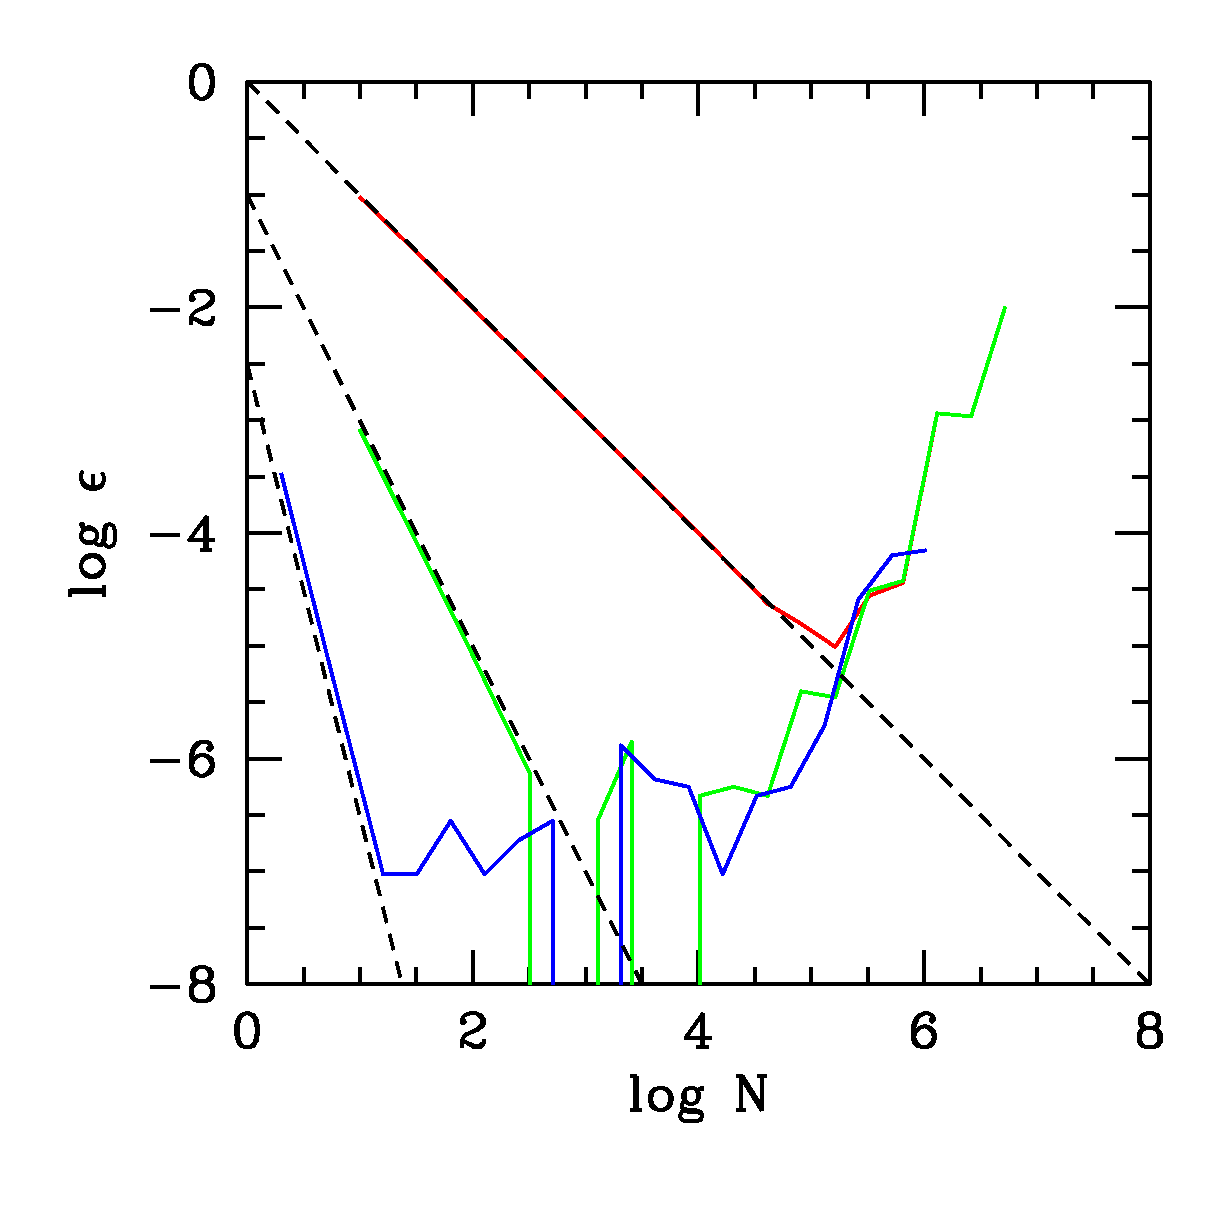
\includegraphics[width=0.4\textwidth]{figure1.ps}
\caption{This figure shows how good my code is.}
\label{figeps}
\end{center}
\end{figure}



\end{document}
